%--------------------------------preamble------------------------------------%
\documentclass[a4paper,10pt]{article}
\usepackage[english]{babel}
\usepackage[utf8]{inputenc}
% use the appendix package
\usepackage{setspace}
\usepackage{appendix}
% 
\include{indentfirst}
% customed definition of the appendix title
\renewcommand\appendix{\par
\setcounter{section}{0}
\setcounter{subsection}{0}
\gdef\thesection{Appendix \Alph{section}}}
%
\usepackage{verbatim}
\begin{comment}
\makeatletter
\renewcommand{\numberline}[1]{%
\settowidth\@tempdimb{#1\hspace{0.5em}}%
\ifdim\@tempdima<\@tempdimb%
  \@tempdima=\@tempdimb%
\fi%
\hb@xt@\@tempdima{\@cftbsnum #1\@cftasnum\hfil}\@cftasnumb}
\makeatother
\end{comment}

%
\usepackage{indentfirst}
\usepackage{verbatim}
% Adjusting line spacing
%\usepackage{setspace}
\addtolength{\parskip}{.4em}
% adding special text style
\usepackage{lettrine} % Big size letter at the begininig of paragraph
% Including math packages
\usepackage{amsmath}
\usepackage{amssymb}
%setlength\LTleft{0pt}
% picture insertion
\usepackage{graphicx}
\usepackage{subfig}
%\usepackage{subcaption}
% userdefined table auto 
\usepackage{longtable,tabularx}
\usepackage{booktabs}
\usepackage{multirow}
\newcommand{\tabincell}[2]{\begin{tabular}{@{}#1@{}}#2\end{tabular}} 

%userdefined caption
\usepackage{caption}

% Biography and references
\usepackage{hyperref}
\hypersetup{
   colorlinks=true,
   linkcolor=blue,
   filecolor=blue,
   urlcolor=blue,
   citecolor=cyan,
}
\usepackage{biblatex}           %Imports bib-latex package
\addbibresource{reference.bib}     %Import the bibliography file

% define paper margin
\usepackage{geometry}
\geometry{left=3.18cm,right=3.18cm,top=2.54cm,bottom=2.54cm}

% define foot and page number
\usepackage{fancyhdr}
\pagestyle{fancy}
\fancyhf{}
\lhead{}
%\rhead{\boldmathseries The performance of new graduates}
\rhead{Draft}
\cfoot{-\hspace{0.5ex}\thepage\hspace{0.5ex}-}
%\rfoot{From:Peter Tang}
\renewcommand{\headrulewidth}{0.4pt}
\renewcommand{\footrulewidth}{0.4pt}

% define title
\title{Boundary Equilibrium bifurcation in Hybrid systems}
\author{Peter Tang \thanks{PhD. candidate in Engineering Mathematics, University of Bristol}}
\date{Dec. 2021}
\begin{document}
	\captionsetup[figure]{labelfont={default},labelsep=period,name={Fig.}}
	\maketitle
	%
	\tableofcontents
	\listoffigures
	\listoftables
	%
	\clearpage
	%
	\section{Base stone case: SDOF impacting oscillator}
	For simplicity, we start from a SDOF impact oscillator. For a conservative SDOF impact oscillator, we would like to start from it to know how the Boundary Equilibrium Bifurcation occurs and the condition for its existence and stability. We suppose that there is a external force $\mu$ to change the equilibrium for + region to - region.  
	\begin{equation}
	m_0 \ddot{X} + c_0 \dot{X} + k X =f
	\end{equation}
	Dividing both sides of the equation above (in time T) with $k$ and letting $X_{st}=\frac{f}{k}$, we can get 
	\begin{equation}
	\frac{\ddot{X}}{\omega^{2}_0}+\frac{c_0}{k}\dot{X}+X=X_{st}
	\label{eq:2}
	\end{equation}
	Meanwhile, take the substitution by $ \displaystyle  \rm{d} t= \omega_0 \rm{d} T$,$ \displaystyle  \bar X=\frac{X}{X_{st}}$ and $ \displaystyle 2\xi=\frac{c_0\omega_0}{k}$, sometimes called damping ratio, we can get a nondimensionalized  equation in a general form
	\begin{equation}
	\ddot{\bar{X}} +2\xi \dot{\bar{X}}+ \bar{X}=1
	\label{eq:nondim Equi1}
	\end{equation} if $f>0$ and 
	\begin{equation}
	\ddot{\bar{X}} +2\xi \dot{\bar{X}}+ \bar{X}=-1
	\label{eq:nondim Equi2}
	\end{equation} if $f<0$.
	where $ \displaystyle \omega_0=\sqrt{\frac{k}{m_0}}$ is the natural frequency of the system.
	At $\bar X=0$ the velocity will be reset by an impact map. 
	
	
	
	\subsection{$f>0$}
	Make translation $U=\bar X-1$, in this case, when the trajectory hits the $\Sigma=\{ U+1=0\}$ the $a(x)>0$ so there is no sticking set.
	\begin{equation}
	\ddot U+2\xi \dot U+U=0
	\label{eq:generalized 1dof equation}
	\end{equation}
	and now the reset map will take pace at $U=-1$. This model and be depicted by fig.\ref{fig:SDof Model}
	\begin{figure}[htpb]
		\centering
		\includegraphics[width= 0.5 \textwidth]{BEB_Explanation/figures/SDOF_model.png}
		\caption{Sketch of the SDOF impact model}
		\label{fig:SDof Model}
	\end{figure}
	
	And the general solution of the Eq. \ref{eq:generalized 1dof equation} will be
	\begin{align}
	U={\rm e}^{-\xi t}\left [U_0\cos{\omega_1 t}+\frac{\dot U_0+\xi U_0}{\omega_1} \sin{\omega_1 t}  \right]\\
	\dot U={\rm e}^{-\xi t}\left[ \dot U_0 \cos{\omega_1 t}-\frac{U_0+\xi \dot U_0}{\omega_1} \sin{\omega_1 t}\right]
	\end{align}
	If the trajectory's starting point is $(U_0,\dot U_0)=(-1,S)$, then 
	\begin{align}
	U={\rm e}^{-\xi t}\left [-\cos{\omega_1 t}+\frac{S-\xi }{\omega_1} \sin{\omega_1 t}  \right]\\
	\dot U={\rm e}^{-\xi t}\left[ S \cos{\omega_1 t}-\frac{\xi S -1}{\omega_1} \sin{\omega_1 t}\right]
	\end{align}
	Suppose that the trajectory will arrive at the $U=-1$ with velocity $S^{'}$ at time $t_1=\frac{\tau_1}{\omega_1}$
	\begin{align}
	-1&={\rm e}^{-\mu \tau_1}\left [-\cos{\tau_1}+\frac{S-\xi }{\omega_1} \sin{\tau_1}  \right]\\
	S^{'}&={\rm e}^{-\mu \tau_1}\left[ S \cos{\tau_1}-\frac{\xi S -1}{\omega_1} \sin{\tau_1}\right]
	\end{align}
	Where $\displaystyle \mu = \frac{\xi}{\omega_1}=\frac{\xi}{\sqrt{1-\xi^2}}$. Thus, we can get S, $S^{'}$ as a function $\tau_1$
	\begin{align}
	S&=-\frac{{\rm e}^{\mu \tau_1}-\cos{\tau_1}-\mu \sin{\tau_1}}{\sqrt{1+\mu^2}\sin{\tau_1}} \label{eq: bounding velocity}\\ \nonumber
	S^{'}&={\rm e}^{-\mu \tau_1}\left[ (\cos{\tau_1-\mu\sin{\tau_1}})S+\sqrt{1+\mu^2}\sin{\tau_1}\right]\\ \nonumber
	&={\rm e}^{-\mu \tau_1} \left[ \frac{-1}{\sqrt{1+\mu^2}\sin{\tau_1}}  ({\rm e}^{\mu \tau_1}\cos{\tau_1}-\mu {\rm e}^{\mu \tau_1}\sin{\tau_1}-\cos^2{\tau_1}+\mu \cos{\tau_1}\sin{\tau_1}-\mu \cos{\tau_1}\sin{\tau_1}+\mu^2\sin^2{\tau_1}) \right. \\ \nonumber 
	& +
	\left. \sqrt{1+\mu^2}\sin{\tau_1} \right]\\ \nonumber
	&=\frac{{\rm e}^{-\mu \tau_1}}{\sqrt{1+\mu^2}\sin{\tau_1}}\left[ -{\rm e}^{\mu \tau_1}\cos{\tau_1}+\mu {\rm e}^{\mu \tau_1}\sin{\tau_1}+\cos^2{\tau_1}-\mu^2\sin{\tau_1}+(1+\mu^2)\sin^2{\tau_1}\right]\\
	&=\frac{{\rm e}^{-\mu \tau_1}-\cos{\tau_1}+\mu \sin{\tau_1}}{\sqrt{1+\mu^2}\sin{\tau_1}}
	\label{eq:hitting velocity}
	\end{align}
	we find that \[ \frac{\rm d S}{\rm d \tau_1}=-\frac{1-{\rm e}^{\mu \tau_1}(\cos{\tau_1}-\mu\sin{\tau_1})}{\sqrt{1+\mu^2}\sin^2{\tau_1}}
	\] and  \[ \frac{\rm d S^{'}}{\rm d \tau_1}= \frac{1-{\rm e}^{-\mu \tau_1}(\cos{\tau_1}+\mu \sin{\tau_1})}{\sqrt{1+\mu^2}\sin^2{\tau_1}}\]
	We introduce the auxiliary function\cite{ANDRONOV1966443}
	\begin{equation}
	\varphi(\tau,\mu)=1-{\rm e}^{\mu \tau}(\cos{\tau}-\mu\sin{\tau}), \; \partial \varphi/\partial{\tau}={\rm e}^{\mu\tau}(1+\mu^2)\sin{\tau}
	\end{equation}
	\begin{figure}
		\centering
		\includegraphics[width=0.6 \textwidth]{BEB_Explanation/figures/auxiliary_fun.png}
		\caption{auxiliary function}
		\label{fig:auxiliary function}
	\end{figure}
	Then we can reorganize the equations above to
	\begin{subequations} \label{eq: reorganization after aux}
		\begin{align}
		S&=-\frac{{\rm e}^{\mu \tau_1}(1-{\rm e}^{-\mu \tau_1}(\cos{\tau_1}+\mu \sin{\tau_1}))}{\sqrt{1+\mu^2}\sin{\tau_1}} = -\frac{{\rm e}^{\mu \tau_1}\varphi(\tau_1,-\mu)}{\sqrt{1+\mu^2}\sin{\tau_1}}  \label{eq: REO S}\\ 
		S^{'}&=\frac{{\rm e}^{-\mu \tau_1}(1-{\rm e}^{\mu \tau_1}(\cos{\tau_1}-\mu \sin{\tau_1}))}{\sqrt{1+\mu^2}\sin{\tau_1}}=\frac{{\rm e}^{-\mu \tau_1}\varphi(\tau_1,\mu)}{\sqrt{1+\mu^2}\sin{\tau_1}}    \label{eq: REO S'} \\
		\frac{\rm d S}{\rm d \tau_1}&=-\frac{\varphi(\tau_1,\mu)}{\sqrt{1+\mu^2}\sin^2{\tau_1}}  \label{eq:REO dSdt} \\
		\frac{\rm d S^{'}}{\rm d \tau_1}&=\frac{\varphi(\tau_1,-\mu)}{\sqrt{1+\mu^2}\sin^2{\tau_1}} \label{eq: REO dS'dt}
		\end{align}
	\end{subequations}
	Thus $S$ is the starting velocity and the $S^{'}$ is the velocity at next intersection point, after some evolution time. Here we consider two different conditions: $(1)f>0$ (admissible equilibrium); $(2)f<0$ (pseudo equilibrium).
	
	\begin{enumerate}
		\item {Case I: $\xi>0$}
		
		For simplicity, we suppose $S>0$, from fig.\ref{fig:auxiliary function}  we know that when $S^{'}=0$ there will be two roots of $\tau_1$ namely $\tau_1^1=0$ and $\tau_1^2=\tau(\mu)\in (\pi,2\pi)$. The non-trivial root $\tau_1^2$ stands for the evolution time. Using Eq.\ref{eq: REO S} we can get the critical value for \[S_{cr}=-\frac{{\rm e}^{\mu \tau(\mu)}\varphi(\tau(\mu),-\mu)}{\sqrt{1+\mu^2}\sin{\tau(\mu)}}\]
		
		It means that when $S<S_{cr}$ the path will eventually be attracted to the origin and only those cases with larger S will have the chance to hit the boundary $U=-1$ and continue the evolution loop.
		\begin{equation} 
		S=S_{cr}+\int_{\tau(\mu)}^{\pi}\frac{\rm d S}{\rm d \tau_1} \rm d \tau_1
		\label{eq:intS}
		\end{equation}
		According to eq.\ref{eq:REO dSdt} we can get eq.\ref{eq:intS} and obviously when $\tau_1$ varies from 0 to $\pi$, S will vary from 0 to $-\infty$ and vary from 0 to $+\infty$ when $\tau_1$ varies from $\tau(\mu)$ to $\pi$; in another word,
		\begin{align}
		\lim_{S \rightarrow S_{cr}+}\tau_1&=\tau(\mu)^-, \; \lim_{S \rightarrow +\infty}\tau_1=\pi^+ 
		\label{eq:admissible eq evolution}
		\\
		\lim_{S \rightarrow -0}\tau_1&=0^+,\;\lim_{S \rightarrow -\infty}\tau_1=\pi^-
		\label{eq:pseudo eq evolution}
		\end{align}
		
		In our case, we assume that the path of this system starts with a positive velocity S and arrives the boundary $U=-1$ with a negative velocity $S^{'}$, and obviously the relationship between the $S$ and $S^{'}$ is implicitly defined by the eq.\ref{eq: reorganization after aux}. However, based on $\displaystyle |\frac{\rm d S^{'}}{\rm d S}|=\frac{\varphi(\tau_1,-\mu)}{\varphi(\tau_1,\mu)}>0$ and, $\tau_1 \in (\pi,\tau(\mu))$ with initial point $S^{'}(0)=0,\;S=S_{cr}$. As $S\rightarrow+\infty$, there will be an asymptotic result
		%
		
		\begin{align}
		&\lim_{S \rightarrow +\infty}\ |\frac{S^{'}}{S}|=\lim_{\tau_1\rightarrow \pi^+} |-{\rm e}^{-2\mu\tau_1}\frac{\varphi(\tau_1,\mu)}{\varphi(\tau_1,-\mu)}|=\lim_{\tau_1\rightarrow \pi^+} |-{\rm e}^{-2\mu\tau_1}{\rm e}^{\mu \pi}|= {\rm e}^{-\mu \pi}\\
		&\lim_{S \rightarrow +\infty} |S^{'}|-{\rm e}^{-\mu \pi}S={\rm e}^{-\mu \pi}
		\label{eq: asymptotic line}
		\end{align}
		%
		and 
		\begin{align}
		\nonumber
		\frac{|\rm d S^{'}/\rm d S|}{\rm dS}=\frac{\rm d \frac{\varphi(\tau_1,-\mu)}{\varphi(\tau_1,\mu)}} {\rm d \tau_1} \frac{1}{\rm d S/\rm d \tau_1}\\ 
		= \frac{2(1+\mu^2)^{\frac{3}{2}} \sin^3{\tau_1} (\sinh{\mu \tau_1} - \mu \sin{\tau_1})}{\phi^3(\tau_1,\mu)}<0
		\end{align}
		\begin{figure}[htbp]
			\centering
			\subfloat[$0<\xi<1$]{\includegraphics[height=0.3 \textheight, width = 0.5 \textwidth]{BEB_Explanation/figures/SDOF_impact_S.png}
			}
			\quad
			\subfloat[$\xi=0$]{\includegraphics[width = 0.45 \textwidth]{BEB_Explanation/figures/SDOF_impact_mu0.png}
			}
			\quad
			\subfloat[$\xi<0$]{\includegraphics[width = 0.45 \textwidth]{BEB_Explanation/figures/SDOF_impact_US.png}
			}
			\caption{Three cases : $I:\,0<\xi<1;\;II:\,\xi=0;\;III:\,\xi<0$}
			\label{fig: three cases for mu}
		\end{figure}
		Thus we have a map $S_0\rightarrow S^{'}_0=-P_0*S_0 \rightarrow S_1=-r*S^{'}_0=r*P_0*S_0\rightarrow S^{'}_2=-P_1*S_1\rightarrow ...$. We can plot this map fig.\ref{fig: three cases for mu}.a. It can be seen that there is no stable limit cycle.
		
		\item{Case II: $\xi<0$}
		
		
		In this case,  given a bounding velocity, the return time $\tau_1$ will be given, $S^{'}>S>0$ due to the divergent motion.  $S=0$ is the critical value and the $\tau(\mu)$
		is solved by eq.\ref{eq: REO S}, which is easily shown the same as the result in the previous case. Substitute the $\tau(\mu)$ into eq.\ref{eq: REO S'} we can get $S^{'}_{cr}$. And the asymptotic's slope is the same expression as in eq.\ref{eq: asymptotic line}. The impact map is still $S_{k+1}=-rS^{'}_{k}$, and the composed map will be the Fig.\ref{fig: three cases for mu}. It shows that if and only if $1/r>{\rm e}^{-\mu \pi}$ will there be a limit cycle and even globally stable.
		\item{Case III: $\xi=0$}
		
		Interesting enough, in this case, the equilibrium is right located on the boundary, and  $r{\rm e}^{\mu \pi}$ means there will be LCO with any amplitude, $r<1$ will lead to convergence to a LCO with amplitude 1 and $r>1$ will lead to divergent motion.
		
	\end{enumerate}
	
	\subsection{$f<0$} 
	When
	$f<0$, the equilibrium is a pseudo type, the steady response will be an equilibrium in sticking set.
	When $f$ changes from negative to positive, the equilibrium will firstly be a pseudo equilibrium ($f<0$), then boundary equilibrium ($f=0$), finally to an unstable admissible equilibrium ($f>0$). The results can be show in Fig.\ref{fig:SDOF BEB} 
	\begin{figure}[h!]
		\centering
		\includegraphics[width= 0.6 \textwidth]{BEB_Explanation/figures/SDOF_BEB.eps}
		\caption{Boundary equilibrium bifurcation}
		\label{fig:SDOF BEB}
	\end{figure}
	The amplitude's linear dependence on $\mu$ can be easily  explained by rescaling in Eq.\ref{eq:nondim Equi1} and Eq.\ref{eq:nondim Equi2}.
	\section{3 Dimensional Hybrid System}
	\begin{enumerate}
		\item[step0:]  To start with a general impacting Hybrid system, the system's local Jacobian $\mathbf{A}$, local switching manifold $H(\mathbf{x}) = \mathbf{Cx}=0$ and the reset map vector $\mathbf{B}$.  Assuming the kernel of $C$ is $[v_2,\cdots,v_n]$. Some constraints as 
		\[ CB = 0 \]
		So that $B = \sum_{i=2}^{n} b_i v_i$, we can always rescale the $b_i$ with $b_i = b_i  |C|$ and $C = C / |C|$ to make $C$ a unit vector.
 		\item[step1:] For a general $\mathbf{C}$, we can  transform the $\mathbf{A}$ to a generalized Li\'enard form $\hat{\mathbf{A}}$ with $n$ unknown parameters, while at the same time keep the direction of $C$ with $n-1$ parameters to describe it. And $B = OZ^{-1} B$.
 		\item[ step2:] Then we use it with its kernel to construct a transformation matrix $\mathbf{P}$ (normal orthogonal basis) to rewrite the system in a new basis.  And $P^{-1}C = \hat{C} = e_1$. Now the $\hat{B} = P^{-1} B = P^T B = \sum_{i=2}^{n} b_i e_i$.
	\end{enumerate}

	 n-D dynamical system defined by an ODE like above mentioned set up, there will be $n + 2(n -1)$ parameters to define a such system, this is a reason why the hybrid system become so complex.
	 
	 so the results in step2 is of a general case, and especially for a mechanical system, $C$ is the first standard basis in $\mathbb{R}^n$, which means the system's codimension is reduced by $n-1$ but remains $n + n -1$.  While $C$ could be more complex and defined by another $n-1$ parameters. 
	 
	 Therefore Lets consider a first case with $C = e_1^T$,	for the original system, with
	 \begin{equation}
	 	\begin{cases}
	 	\dot{\mathbf{x}} =\mathbf{A} \mathbf{x} , ~~ H(\mathbf{x}) > 0 \\
	 	\mathbf{x}^+ = \mathbf{(I - BCA)}  \mathbf{x}^-, ~~ H(\mathbf{x}) = 0
	 	\end{cases}
	 \end{equation}	where $H(\mathbf{x})$ is a defined discontinuity manifold and here we treat it as a plane or super-plane in state space.
We assume  eigenvalues $\lambda_1, \lambda_2, \lambda_3$ and $\lambda_3 \neq 0$, which is the real eigenvalue, then we can transform it into a Li\'enard form as 
 \[ M = P^{-1} A P = Q^{-1} \begin{bmatrix}
 	\lambda_1 & 0 & 0\\ 0 & \lambda_2 & 0 \\ 0 & 0 & \lambda_3
 \end{bmatrix} Q= \begin{bmatrix}
 	a_1 & 1 & 0\\ a_2 & 0 & 1 \\ a_3 & 0 & 0
 \end{bmatrix}, B = P^{-1}B_0 = \begin{bmatrix}
 	0\\b_2\\b_3
 \end{bmatrix}, CP =C \]  

we can redefine the system by rescale the time  ${\rm d} t = {\rm d} \tau / |\lambda_3|$
	\begin{equation}
	\begin{cases}
	\dot{\mathbf{x}} =\frac{\mathbf{A}}{|\lambda_3|}\mathbf{x} , ~~ H(\mathbf{x}) > 0 \\
	\mathbf{x}^+ = \mathbf{R}(\mathbf{x}^-), ~~ H(\mathbf{x}) = 0
	\end{cases}	
	\end{equation}
The \[ \hat{M} = P^{-1} \frac{\mathbf{A}}{|\lambda_3|} P = \frac{1}{|\lambda_3|}Q^{-1} \begin{bmatrix}
	\lambda_1 & 0 & 0\\ 0 & \lambda_2 & 0 \\ 0 & 0 & \lambda_3
\end{bmatrix} Q= \begin{bmatrix}
	\hat{a}_1 & 1 & 0\\ \hat{a}_2 & 0 & 1 \\ \hat{a}_3 & 0 & 0
\end{bmatrix}, \hat{B} = \begin{bmatrix}
	0\\b_2\\b_3
\end{bmatrix} \] 
Then the redefined system  via $x = Py$ is 
\begin{equation}
	\begin{cases}
		\dot{\mathbf{y}} =P^{-1} \frac{\mathbf{A}}{|\lambda_3|} P \mathbf{y} = \hat{M} \mathbf{y} , ~~ H(\mathbf{y}) > 0 \\
		\mathbf{y}^+ = P^{-1} \mathbf{(I - B_0 C \frac{\mathbf{A}}{|\lambda_3|} )}  P \mathbf{y}^- =\mathbf{(I - \hat{B} C \hat{M}) }\mathbf{y}^- , ~~ H(\mathbf{y}) = 0
	\end{cases}	
\end{equation}
	
Then the system is defined by $\{ \hat{\lambda}_1, \hat{\lambda}_2,  \hat{\lambda}_3= \pm 1, \hat{b}_2 = 1.75, \hat{b}_3 \}$
\[\hat{a}_1 = \hat{\lambda}_1+\hat{\lambda}_2+\hat{\lambda}_3, \hat{a}_2 = \hat{\lambda}_1 \hat{\lambda}_2 + \hat{\lambda}_1 \hat{\lambda}_3 + \hat{\lambda}_2 \hat{\lambda}_3, \hat{a}_3 = \hat{\lambda}_1 \hat{\lambda}_2 \hat{\lambda}_3\]

Now we reduced the dimension of parameter space to $3$ and to understand the system by tuning the $\hat{\lambda}_1, \hat{\lambda}_2,  \hat{b}_3$.
\begin{enumerate}
	\item[$\hat{\lambda}_3 = 1$]: we can still say this can be divided by if the $\hat{\lambda}_1, \hat{\lambda}_2$ are real or complex;
	\begin{itemize}
		 \item[real:]  $ (1)\hat{\lambda}_1 = \hat{\lambda}_2; (2) \hat{\lambda}_1 > \hat{\lambda}_2; (3) \hat{\lambda}_1 < \hat{\lambda}_2;$ 
		 \item[complex:] $\hat{\lambda}_1 = \alpha + i \beta$
	\end{itemize}
	\item[$\hat{\lambda}_3 = -1$]: 
	\begin{itemize}
		\item[real:]  $ (1)\hat{\lambda}_1 = \hat{\lambda}_2; (2) \hat{\lambda}_1 > \hat{\lambda}_2; (3) \hat{\lambda}_1 < \hat{\lambda}_2;$ 
		\item[complex:] $\hat{\lambda}_1 = \alpha + i \beta$
	\end{itemize}

\end{enumerate}
In a 3D parameter space, we use the Montel-carol method to find the system's LCO. Given a point $[\hat{\lambda}_1, \hat{\lambda}_2,  \hat{b}_3]$ if there is an LCO use (1 PSE) blue solid circle for stable one and blue empty circle for unstable one (2ASE) red solid circle for stable one and red empty circle for unstable one ; nothing for a point with no LCO.


	According to the sign of the velocity $\mathcal{L}_F(H)(x)$ we can define a minus set $\{\Sigma^-|v<0,H(\mathbf{x}) = 0\}$, a positive set $\{\Sigma^+|v>0,H(\mathbf{x}) = 0\}$ and tangent set $\{\Sigma^0|v=0,H(\mathbf{x}) = 0\}$ on the manifold $\{\Sigma|H(\mathbf{x}) = 0\}$. The truth is that the flow will bring every point in positive set to minus set, while the reset map will reset the points in $\Sigma^-$ to $\Sigma^+$. Then there is a composed map defined on both sets and we say a limit cycle exist when the composed map has fix point(s) with period $T^* = \tau_F + \tau_R$, where the evolution time of the flow to get the discontinuity manifold again is $\tau_F$, and $\tau_R$ for the reset map respectively. 
	For simplicity but generality, further we define $H(\mathbf{x}) = C \mathbf{x} =0$ and $C = [1,0,\cdots,0]_{n,1}$ is the normal vector, where we can  always transform the coordinates to reach this.  
	
	For a 3-D linear ODE system, there are two cases of the eigenvalues: 1) three real eigenvalues; 2) a pair of conjugate complex eigenvalues ($-\alpha \pm \beta i$) and a real one $-\lambda$. We will focus on the second case which is of more physical meaning. Specifically, the eigenvector of the real eigenvalue $\lambda$ is $\mathbf{v}_3$. Here we want to give the criteria for existence and stability of the LCO in the 3-D hybrid system. There are different cases in need of careful treatment: Is the equilibrium located on the $\Sigma$? If not, Is there any pseudo equilibrium (if yes, how about the stability)? Is the $\mathbf{v}_3 $ in parallel to the $\Sigma$? So there should be 4 main different cases and we will treat them in turn.
	
	\paragraph{Case I: Equilibrium on the Boundary}
	$\dot{\mathbf{x}} =\mathbf{A}\mathbf{x}$. In this case the equilibrium is on the boundary. And the border distinguishing the positive and minus sets is $\Sigma^0 = \{(x_2,x_3)|a_{12}x_2+ a_{13}x_3+f_1=0\}$, or $l_3$ with the direction vector $\mathbf{V}_{l3} = [0,\frac{a_{13}}{\sqrt{a_{12}^2+a_{13}^2}},\frac{-a_{12}}{\sqrt{a_{12}^2+a_{13}^2}}]^{\top} $. %We should clarify the stability of it.
	In essence, the reset map will flip the point in minus set and expand/contract along the perpendicular direction to $l_3$ and make translation along the $l_3$. Now we construct the reset map as following;
	
	For a state $[0,y_0,z_0]^{\top}$ in minus set, we know the $r^- = \frac{|a_{12}y_0+a_{13}z_0+f_1|}{\sqrt{a_{12}^2+a_{13}^2}}$ and  unit vector vertical to the line $l_3$ as $\mathbf{P}_{l3} = [0,\frac{a_{12}}{\sqrt{a_{12}^2+a_{13}^2}},\frac{a_{13}}{\sqrt{a_{12}^2+a_{13}^2}}]^{\top}$, $z^- = [0,y_0,z_0]^{\top} \mathbf{V}_{l3} $
	
	So the reset map 
	$$R \circ
	\begin{bmatrix}
	0\\y_0\\z_0
	\end{bmatrix} = 
	\begin{bmatrix}
	0\\y_0\\z_0
	\end{bmatrix} + \phi_1(r^-,z^-) \mathbf{P}_{l3}+\phi_2(r^-,z^-) \mathbf{V}_{l3}
	$$
	
	\subparagraph{(1) $\mathbf{v}_3$ in parallel with the $\Sigma$}
	In this case, actually the $\mathbf{v}_3$ is on the $\Sigma$ and the line $l_3$ through the origin (equilibrium) is in the derection of $\mathbf{v}_3 = \mathbf{V}_{l3}$, which seperates the discontinuity manifold to $\Sigma^+$ and $\Sigma^-$.We define the distance between the point of trajectory and the axis as $\mathbf{r}$, the eigen coordinnate along $\mathbf{v}_3$ as $z$.
	\begin{equation}
	\begin{bmatrix}
	{r}^-\\{z}^-
	\end{bmatrix}
	=
	\begin{bmatrix}
	{\rm e}^{-\alpha \tau_F} & 0\\ 0 & {\rm e}^{-\lambda \tau_F}
	\end{bmatrix} \begin{bmatrix}
	{r}^+\\{z}^+
	\end{bmatrix}
	\end{equation}
	where $\tau_F =\frac{\pi}{\beta}$ (the discontinuity surface divides the phase evenly) and we define the reset map as \[ \mathbf{R} \circ \begin{bmatrix}
	{r}^-\\{z}^-
	\end{bmatrix} = \begin{bmatrix}
	{R}_1(r^-,z^-)\\{R}_2(r^-,z^-)
	\end{bmatrix}\]
	
	Suppose we find a LCO starting from $[r^+_*;z^+_*]$ ending at $[r^-_*;z^-_*]$, satisfying  the
	$$R_1(r^-_*,z^-_*) = {\rm e}^{\alpha \tau_F} r^-_*;~ R_2(r^-_*,z^-_*) = {\rm e}^{\gamma \tau_F} z^-_*$$
	and the Jacobi matrix of the composed map is 
	\begin{equation}
	J = \begin{bmatrix}
	b_{11}& b_{12}  \\  b_{21} & b_{22}
	\end{bmatrix} 
	\begin{bmatrix}
	{\rm e}^{-\alpha \tau_F} & 0\\ 0 & {\rm e}^{-\lambda \tau_F}
	\end{bmatrix}
	\end{equation}
	where 
	$b_{11} = \frac{\partial {R_1}}{\partial r}|_{r_*^-}$, $b_{12} = \frac{\partial {R_1}}{\partial z}|_{z_*^-}$, $b_{21} = \frac{\partial {R_2}}{\partial r}|_{r_*^-}$, $b_{22} = \frac{\partial {R_2}}{\partial z}|_{z_*^-}$.
	\subparagraph{(2) $\mathbf{v}_3$ intersecting with the $\Sigma$} 
	We ignore the special case where the $\mathbf{v}_3$ is perpendicular to the $\Sigma$ in which the $\tau_F = 2\pi$ so that the region of the evolution time $\tau_F$ is $(\pi,2\pi)$.
	There will be two implicit defined functions to describe the relationship.
	
	In this case 
	\paragraph{Case II: Equilibrium not on the Boundary}
	$\dot{\mathbf{x}} =F(\mathbf{x})=\mathbf{A}\mathbf{x} +\mathbf{f}$
	\subparagraph{(1) $\mathbf{v}_3$ in parallel with the $\Sigma$}
	Same with the 1DOF case in finding the condition for $R_1(r)$ map, and only when the condition $R_2(z^-_*) = z^-_* {\rm e}^{\tau_F}$ is simultaneously true can a LCO orbit exist.
	\subparagraph{(2) $\mathbf{v}_3$ intersecting with the $\Sigma$} 
	Suppose the $\mathbf{v}_3$ intersect with the $\Sigma$ at point E, and the separating line $l_3$ will be through this point. 
	
	
	The procedure to construct a desired system:
	
	For a general system $\dot{X}= A(X-X_0)$, we can find its eigenvalues, $\alpha \pm i \beta$, $\lambda$ and  eigenvectors $v_i$. Especially we define the $v_3$ is the eigenvector of $\lambda$. For the convenience of observation, we can always transform the $\mathbf{v}_3$ to be in parallel with the $XoZ$ plane of the inertial frame, without loss of generality.
	
	We define the relative angle between the $\mathbf{v}_3 $ and the normal vector $ \mathbf{n} = C^{\top}$ is $\theta$, and the general rotation matrix 
	\begin{equation}
	\bar{R}(\mathbf{l},\theta) = \mathbf{I}+ \sin(\theta) [\mathbf{l}]_{\times} + (1-\cos(\theta))[\mathbf{l}]_{\times}^2
	\label{eq:rotation matrix}
	\end{equation}
	where 
	$$
	[\mathbf{l}]_{\times} = \begin{bmatrix}
	0 		 & -{l}_z  & {l}_y\\
	{l}_z    & 		0  & -{l}_x\\
	-{l}_y   &  {l}_x  & 0
	\end{bmatrix}
	$$
	and $\mathbf{l}$ is the axis.
	\begin{enumerate}
		\item  Transform to canonical forms in align with above 4 lemmas.
		
		(1) Let $X_0=0$ and if $0< \theta < \frac{\pi}{2}$ 
		and we can rotate the system by  $\bar{R}(\mathbf{l}_0,\frac{\pi}{2}-\theta)$ in which $\mathbf{l}_0 =  \mathbf{n} \times \mathbf{v}_3 $. In the end, we can get a new $\mathbf{v}_3$ satisfying $\mathbf{v}_3 \perp \mathbf{n}$; 
		
		(2) $X_0=0$ and $\mathbf{n} \cdot \mathbf{v}_3\neq 0$; If else we can rotate the system by $\bar{R}(-\mathbf{l}_0,\theta)$;
		
		(3) Set $X_0=[-1,y_0,z_0]^{\top}$ and if $0< \theta < \frac{\pi}{2}$ 
		and we can rotate the system by  $\bar{R}(\mathbf{l}_0,\frac{\pi}{2}-\theta)$ in which $\mathbf{l}_0 =  \mathbf{n} \times \mathbf{v}_3 $. In the end, we can get a new $\mathbf{v}_3$ satisfying $\mathbf{v}_3 \perp \mathbf{n}$;
		
		(4) $X_0=[-1,y_0,z_0]^{\top}$ and $\mathbf{n} \cdot \mathbf{v}_3 \neq 0$; If else we can rotate the system by $\bar{R}(-\mathbf{l}_0,\theta)$.
		\item After the above manipulation, we refresh our matrix $A$, relative angle $\theta$.
		We give our special four canonical examples:
		
		(1) $A = \begin{bmatrix}
		\alpha & \beta & 0\\
		- \beta & \alpha & 0\\
		0 & 0 & \lambda
		\end{bmatrix}$, $X_0=\mathbf{0}$
		
		(2) $A =\begin{bmatrix}
		\cos(\theta) & 0 & -\sin(\theta)\\
		0& 1& 0\\
		\sin(\theta) & 0 & \cos(\theta)
		\end{bmatrix} 
		\begin{bmatrix}
		\alpha & \beta & 0\\
		- \beta & \alpha & 0\\
		0 & 0 & \lambda
		\end{bmatrix}
		\begin{bmatrix}
		\cos(\theta) & 0 & \sin(\theta)\\
		0& 1& 0\\
		-\sin(\theta) & 0 & \cos(\theta)
		\end{bmatrix} $, $X_0=\mathbf{0}$
		
		(3) $A = \begin{bmatrix}
		\alpha & \beta & 0\\
		- \beta & \alpha & 0\\
		0 & 0 & \lambda
		\end{bmatrix}$, $X_0=[-1,0,0]^{\top}$
		
		(4) $A =\begin{bmatrix}
		\cos(\theta) & 0 & -\sin(\theta)\\
		0& 1& 0\\
		\sin(\theta) & 0 & \cos(\theta)
		\end{bmatrix} 
		\begin{bmatrix}
		\alpha & \beta & 0\\
		- \beta & \alpha & 0\\
		0 & 0 & \lambda
		\end{bmatrix}
		\begin{bmatrix}
		\cos(\theta) & 0 & \sin(\theta)\\
		0& 1& 0\\
		-\sin(\theta) & 0 & \cos(\theta)
		\end{bmatrix} $, $X_0=[-1,0,0]^{\top}$
		
		
		
	\end{enumerate}
	For a system (in the forms given above) like $\dot{\mathbf																																														 {x}} =  \mathbf{A} \mathbf{x}$ with initial condition $X_0 = [x_0,y_0,z_0]^{\top}$ where 
	$$A_J={P}^{-1} A P= \begin{bmatrix}
	\alpha & \beta & 0\\
	- \beta & \alpha & 0\\
	0 & 0 & \lambda
	\end{bmatrix}
	$$  and $P = I$(case (1),(3))  or $P = \begin{bmatrix}
	\cos(\theta) & 0 & \sin(\theta)\\
	0& 1& 0\\
	-\sin(\theta) & 0 & \cos(\theta)
	\end{bmatrix}$(case (2),(4)).
	\subsection{Virtual equilibrium cases}
	We focus our attention on the virtual equlibrium cases, where $X_0=[-1,0,0]^{\top}$.
	
	The solution will be $\mathbf{x}-X_0 = {\rm e}^{A_J t}(\mathbf{x}_0 - X_0)$, and we probe into the components of the solution 
	\begin{align}
	\nonumber
	x_1+1 &= \left(\cos^{2}(\theta) {\rm e}^{\alpha t} \cos (\beta t)+\sin^{2}(\theta) {\rm e}^{\lambda t} \right)(x_0+1) \\ \nonumber
	&+ \left(\cos(\theta) {\rm e}^{\alpha t} \sin(\beta ) \right) y_0 \\	
	&+ \left({\rm e}^{\alpha t} \cos(\beta t)-{\rm e}^{\lambda t} \right)\cos(\theta) \sin(\theta)  z_0
	\\  
	y_1 &={\rm e}^{\alpha t} (-\cos(\theta)  \sin(\beta t) (x_0 +1) + \cos (\beta t) y_0 -\sin(\theta)  \sin (\beta t) z_0)
	\\ \nonumber
	z_1 &= \left({\rm e}^{\alpha t} \cos(\beta t)-{\rm e}^{\lambda t} \right)\cos(\theta) \sin(\theta)  (x_0+1)\\ \nonumber
	& -\sin(\theta) {\rm e}^{\alpha t} \sin (\beta t) y_0 \\ 
	& + \left(\sin^{2}(\theta) {\rm e}^{\alpha t} \cos (\beta t)+\cos^{2}(\theta) {\rm e}^{\lambda t} \right) z_0  
	\end{align}
	we know the initial point departures from the positive set so $x_0 = 0$ and arrive at $x_1=0$. 
	\subsubsection{$\theta = 0$} 
	The previous aolution equations will be the same form in the SDOF case (degenerated case):
	\begin{align}
	0 &=-1+{\rm e}^{\alpha t_1} \left(  \cos (\beta t_1) +  \sin(\beta t_1)y_0  \right) 
	\\
	y_1 &=  {\rm e}^{\alpha t_1} \left( -\sin(\beta t_1)  + \cos (\beta t_1) y_0 \right)
	\\
	z_1 &= {\rm e}^{\lambda t_1} z_0
	\end{align}
	This case we can solve the semi-Poincar{\'e} map ($0<t_1<\frac{\pi}{\beta}$) 
	\begin{align}
	\frac{r^+}{r^-} & =\frac{\left(\cos(\beta t_1) \beta-\beta {\rm e}^{\alpha t_1}+\alpha \sin(\beta t_1)\right) {\rm e}^{\alpha t_1}}{\left(\cos(\beta t_1) \beta-\alpha \sin(\beta t_1)\right) {\rm e}^{\alpha t_1}-\beta} \\
	\frac{z^+}{z^-} &= {\rm e}^{\lambda t_1}
	\end{align}
	with 
	$$\lim_{t_1\rightarrow \frac{\pi^-}{\beta}} \frac{r^+}{r^-} = {\rm e}^{\frac{\pi \alpha}{\beta}}$$ and $$\lim_{t_1\rightarrow 0^+} \frac{r^+}{r^-} = 1$$
	especially, $\frac{{\rm d}^2 r^+ / r^-}{{\rm d} t^2}<0$.
	So according to the theorem in previous section, we know we can define a $\phi_1(r^-,z^-) = (1+R_r) r^-,~(1<R_r< {\rm e}^{-\frac{\pi \alpha}{\beta}})$ to get a stable LCO, while $\phi_2(r^-,z^-)$ can be independently defined.
	
	
	\subsubsection{$0<\theta < \frac{\pi}{2}$} 
	 In his case we can solve the semi-Poincar{\'e} map ($0<t_1<\frac{\pi}{\beta}$) 
	\begin{align}
	\frac{r^+}{r^-} & =\frac{a_1 {y_0}+a_2{z_0}+a_3}
	{{\rm e}^{\lambda t} \left(1-{\rm e}^{(\alpha -\lambda) t} \cos(\beta t)\right) 
		\left[\cos(\theta) \beta {y_0}+(\alpha-\lambda) \cos(\theta)^{2}+{z_0} (\alpha-\lambda) \sin(\theta) \cos(\theta)+\lambda
		\right]
	} \\
	\frac{z^+}{z^-} &= \frac{b_1 y_0 + b_2 z_0 +b_3}
	{-\cos(\theta) {\rm e}^{\lambda t_1} 
		\left(
		1- {\rm e}^{(\alpha - \lambda) t_1} \cos(\beta t_1)
		\right) 
		\left( 
		\sin(\theta) (\alpha-\lambda){y_0}-\beta {z_0} \right)
	}
	\end{align}
	where 
	$$
	a_1=\beta \cos(\theta) {\rm e}^{2 \alpha t_1} \left(1 {\rm e}^{(\lambda-\alpha) t_1} \cos(\beta t_1)\right)
	$$
	$$
	a_2 =-{\rm e}^{2\lambda t_1} \sin(\theta) \cos(\theta) (\alpha-\lambda) \left(1-\cos(\beta t_1) {\rm e}^{(\alpha-\lambda) t_1} \right)
	$$
	$$
	a_3 = {\rm e}^{\lambda t_1} 
	\left(
	(\alpha - \lambda)\sin^2(\theta) {\rm e}^{\lambda t_1} - \alpha 
	\right) 
	\left(
	1 - {\rm e}^{(\alpha - \lambda) t_1} \cos(\beta t_1)
	\right) + \beta \sin(\beta t_1) {\rm e}^{\alpha t_1} ({\rm e}^{\lambda t}- 1)
	$$
	$$
	b_1= \sin(\theta) \cos(\theta) {\rm e}^{2 \alpha t_1} 
	\left(
	1 -{\rm e}^{(\lambda-\alpha) t_1} \cos(\beta t_1)
	\right)
	$$
	$$
	b_2= \beta \cos(\theta) {\rm e}^{2 \lambda t_1}
	\left(
	1 -{\rm e}^{(\alpha-\lambda) t_1} \cos(\beta t_1)
	\right)
	$$
	$$
	b_3= \sin(\theta) {\rm e}^{\lambda t_1} 
	\left({\rm e}^{\lambda t}-1\right) 
	\left[
	(\alpha-\lambda) \sin(\beta t) {\rm e}^{(\alpha-\lambda) t_1}-\beta \left(1-{\rm e}^{(\alpha-\lambda) t_1} \cos(\beta t_1)\right) 
	\right]
	$$
	and the evolution time $t_1$ is determined by $y_0,~,z_0$ and the equation
	\begin{equation}
	\cos^2(\theta) {\rm e}^{\alpha t_1} \cos(\beta t_1)+\sin^2 (\theta) {\rm e}^{\lambda t_1}+\cos(\theta) {\rm e}^{\alpha t_1} \sin(\beta t_1) y_0-\cos(\theta) \sin(\theta) {\rm e}^{\lambda t_1}\left[1 - {\rm e}^{(\alpha-\lambda) t_1} \cos(\beta t_1)\right] z_0 =1
	\label{eq:evolution time governing equation}
	\end{equation}
	We should notice that when $(0,y_0,z_0)$ is on the line $a_{12} y_0 + a_{13} z_0 + f_1 = C$, which is in parallel with zero velocity line $l_3$. Specifically, constant $C$ is greater than 0 and determines the distance to the line $l_3$. 
	
	So we can get 
	\begin{equation}
	{y_0}=\frac{(-\alpha+\lambda) \cos(\theta)^{2}-(\alpha-\lambda) \sin(\theta) \cos(\theta){z_0} +C-\lambda}{\beta \cos(\theta)}
	\label{eq:simplified online y0}
	\end{equation}
	Meanwhile, there is a common term $(\alpha - \beta)$ in above equations, so we discuss two cases:
	\begin{enumerate}
		\item $\alpha = \lambda$
		
		By substituting Eq.\ref{eq:simplified online y0} to Eq.\ref{eq:evolution time governing equation} we can get 
		\begin{align}
			\nonumber
			{z_0} &=-\frac{\beta {\rm e}^{-\lambda t}-\cos(\theta)^{2} \cos(\beta t) \beta+(-C+\lambda) \sin(\beta t)+\cos(\theta)^{2} \beta-\beta}{\beta \sin(\theta) \cos(\theta) (\cos(\beta t)-1)}\\
			&=\cot(\theta)+\frac{\beta ({\rm e}^{-\lambda t}-1)+(-C+\lambda) \sin(\beta t)}{\beta \sin(\theta) \cos(\theta) (1-\cos(\beta t))}
			\label{eq:simplified online z0}
		\end{align}
	\begin{align}
		\nonumber
	{y_0} &=\frac{\sin(\theta) \cos(\theta) \cos(\beta t) {z_0}-\sin(\theta) \cos(\theta) {z_0}-\cos(\theta)^{2} \cos(\beta t)+\cos(\theta)^{2}-1+{\rm e}^{-\lambda t}}{\cos(\theta) \sin(\beta t)} \\
	&=
	-\frac{(1-\cos(\beta t))\sin(\theta)}{\sin(\beta t) } ~ ({z_0}-\frac{{\rm e}^{-\lambda t}-1+\cos(\theta)^{2} (1-\cos(\beta t))}{(1-\cos(\beta t)) \sin(\theta) \cos(\theta)})
	\label{eq:retuning time controlled y0}
	\end{align}
	and $z_0$ is anywhere on the plane $x=0$, so $z_0 \in (-\infty,+\infty),~y_0 \in (\frac{-\lambda}{\beta \cos(\theta)},+\infty) $. Actually, from Eq.\ref{eq:simplified online z0} we can get:
	when $y_0$ is a limited positive number
	$$
	\lim_{t \rightarrow 0^+} z_0 = -\infty,~ \lim_{t \rightarrow \frac{ \pi}{\beta}} z_0= \cot(\theta)-\frac{1-{\rm e}^{-\frac{\pi \lambda}{\beta}}}{2 \sin(\theta) \cos(\theta)},~ \lim_{t \rightarrow \frac{2 \pi}{\beta}} z_0= +\infty
	$$
	when $z_0$ is a limited value number and $y_0>0$ must be satisfied:
	$$
	\lim_{t \rightarrow 0^+} y_0 = \frac{-\lambda}{\beta \cos(\theta)} ~ {\rm for} ~z_0 \in (-\infty,+\infty) $$ 
	$$\lim_{t \rightarrow \frac{ \pi}{\beta}^-} y_0= + \infty \text{ for limited }  z_0 $$
	Notice that when $y_0 = + \infty$, $0<t_1<\frac{\pi}{\beta}$ if $- \infty<z_0<\cot(\theta)-\frac{1-{\rm e}^{-\frac{\pi \lambda}{\beta}}}{2 \sin(\theta) \cos(\theta)}$, and $\frac{\pi}{\beta}<t_1<\frac{2\pi}{\beta}$ if $\cot(\theta)-\frac{1-{\rm e}^{-\frac{\pi \lambda}{\beta}}}{2 \sin(\theta) \cos(\theta)}<z_0<+ \infty$.
	
	Meanwhile at the condition $z_0$ is positive infinite large
	$$
	 ~ \lim_{t \rightarrow \frac{2 \pi}{\beta}^-} y_0= -\infty
	$$
	so we know that the evolution time $t_1 \in (0,\frac{2 \pi}{\beta})$
	\begin{equation}
		\frac{r^+}{r^-}=-\left[
		\frac{(-C+\lambda) {\rm e}^{\lambda t}+\lambda}{C}+\frac{\sin(\beta t) \beta \left({\rm e}^{\lambda t}-1\right)}{C (\cos(\beta t)-1)}
		\right]
		\label{eq:ratio_r for case alpha equal lambda}
	\end{equation}
		\begin{align}
		\nonumber
		\frac{z^+}{z^-} &={\rm e}^{\lambda t}+\frac{\sin(\theta) {\rm e}^{\lambda t}-\sin(\theta)}{\cos(\theta) {z_0}}
		\\ \nonumber
		&= 1+(\frac{\tan(\theta)}{z_0}+1) ({\rm e}^{\lambda t}-1)\\
		&=1+\frac{(\left(\beta \cos(\beta t)+\left(C-\lambda\right) \sin(\beta t)\right) {\rm e}^{\lambda t}-\beta) ({\rm e}^{\lambda t}-1)}
		{\left(\cos(\theta)^{2} \cos(\beta t) \beta+\left(C-\lambda\right) \sin(\beta t)-\cos(\theta)^{2} \beta+\beta\right) {\rm e}^{\lambda t}-\beta}
 		\label{eq:ratio_Z for case alpha equal lambda}
		\end{align}
	Now we should try to know the features of $\frac{r^+}{r^-}$ and $\frac{z^+}{z^-}$:
		$$\lim_{t_1\rightarrow \frac{2 \pi^-}{\beta}} \frac{r^+}{r^-} = +\infty,~\lim_{t_1\rightarrow \frac{\pi^-}{\beta}} \frac{r^+}{r^-} = {\rm e}^{\frac{\pi \lambda}{\beta}}-\frac{\lambda(1+{\rm e}^{\frac{\pi \lambda}{\beta}})} {C} ,~\lim_{t_1\rightarrow 0^+} \frac{r^+}{r^-} = 1$$
		 and 
		 $$\lim_{t_1\rightarrow \frac{2 \pi^-}{\beta}} \frac{z^+}{z^-} = {\rm e}^{\frac{2 \pi \lambda}{\beta}},
		 %
		 ~\lim_{t_1\rightarrow \frac{ \pi^-}{\beta}} \frac{z^+}{z^-} = \frac{2 \cos(\theta)^{2}+{\rm e}^{\frac{\pi \lambda}{\beta}}-1}{2 \cos(\theta)^{2}+{\rm e}^{\frac{-\pi \lambda}{\beta}}-1},
		 %
		 ~\lim_{t_1\rightarrow 0^+} \frac{z^+}{z^-} = 1$$
		 We can know for a LCO with limited $z_0$ (physical meaningful), we can only define a $\phi_1(r^-,z^-) = (1+R_r) r^-,~(1<R_r< {\rm e}^{-\frac{\pi \lambda}{\beta}})$ to get a stable LCO, while $\phi_2(r^-,z^-)$ can be independently defined.According to the Eq.\ref{eq:ratio_Z for case alpha equal lambda}, the $z^+/z^-$ can be always equal to 1 when $z_0 = -\tan(\theta)$. 
		 
		 If we set $0\leq \phi_2(r^-,z^-) \leq 1$, in first case, starting from positive value, the coordinates $z_0^k$ will shrink to zero after enough loops $k$, but we should notice that $\dot{z}= -\beta \sin(\theta) y_0<0$, so series $z_0$ will continue to go down less than 0 and then arrive at $-\tan(\theta)$ where $z^+/z^-=1$; in another case, starting from value less than $-\tan(\theta)$, the $z_0^k$ will directly shrink to $z=-\tan(\theta)$; in last case, $\tan(\theta)<z_0^0<0$, $z^+/z^-$ will always be greater than 1, so the  $z_0^k$ will continuously grow in absolute value and converge at $z=-\tan(\theta)$. In a nutshell, the LCO will always hit the boundary with $z_0 = -\tan(\theta)$ in this case, no mater how large the LCO is.
		 
		 If we set $1\leq \phi_2(r^-,z^-) \leq {\rm e}^{\frac{- 2 \pi \lambda}{\beta}}$. The limit cycle oscillation will converge at some value $z_{L2} \leq -\tan(\theta)$. There is another critical value for $z$ which is $z_{cr}= \tan(\theta)( {\rm e}^{-\lambda \tau}-1)$, $\tau$ is controlled by the $y_0,z_0$. Here if starting point $0<z_0^k<z_{cr}$, then $z_0^{k+1}<0$. So, for the $ z_{cr}< z_0 < +\infty$, if the $\phi_2(r^-,z^-)$ can't push $z$ away from 0, the coordinate $z$ will always become negative later on (converging at a point or diverging). $\hfill\blacksquare$
		\item $\alpha \neq \lambda$
		
		By defining $\gamma = \frac{\alpha - \lambda}{\beta}$, $\tau = \beta t$, and substituting Eq.\ref{eq:simplified online y0} to Eq.\ref{eq:evolution time governing equation} we can get 
			\begin{align}
			{z_0} =\cot(\theta)+\frac{\beta ({\rm e}^{-\frac{\lambda}{\beta} \tau}-1)+(-C+\lambda) {\rm e}^{ \gamma\tau} \sin(\tau)}
			{\beta \sin(\theta) \cos(\theta) \varphi_2^{\gamma}(\tau) }
			\label{eq:simplified online z0 case 2}
			\end{align}
			\begin{align}
			\nonumber
			y_0 &=-\frac{\sin(\theta){\rm e}^{-\tau \gamma} \varphi_1^{\gamma}(\tau)}{\sin(\tau)}
			%
			\left(
			{z_0}-\frac{
			 ({\rm e}^{-\frac{\lambda \tau}{\beta}}-1)+\cos(\theta)^{2}  \varphi_1^{\gamma}(\tau)
			}
		    %
			{
			\sin(\theta) \cos(\theta)  \varphi_1^{\gamma}(\tau)
			}
			\right)\\
			&=\frac{
				(C-\lambda) \varphi_1^{\gamma}(\tau)+\beta \gamma ({\rm e}^{- \frac{\lambda \tau}{\beta}}-1)
			}
		%
			{\beta \cos(\theta) \varphi_2^{\gamma}(\tau)
				}
			\end{align}
			where $\varphi_1^{\gamma}(\tau)=1-{\rm e}^{ \gamma\tau}\cos(\tau)$, $\varphi_2^{\gamma}(\tau)=1-{\rm e}^{\tau \gamma}(\cos(\tau)-\gamma \sin(\tau)) = \varphi_1^{\gamma} + \gamma {\rm e}^{\gamma\tau }\sin(\tau)$.
			
			When $\gamma<0$, $\varphi_1^{\gamma}(\tau)>0$ and $\varphi_2^{\gamma}(\tau)>0$ for $\tau \in (0, 2 \pi)$;
			Otherwise $\gamma >0$, $\varphi_1^{\gamma}(\tau)$  has two non-trivial roots, namely $\tau_c^1(\gamma)_1$and  $\tau_c^1(\gamma)_2$, and $\varphi_2^{\gamma}(\tau)$ has one non-trivial root  $\tau_c^2(\gamma)$.
			$\frac{\partial \varphi_2(\tau)}{\partial \tau}={\rm e}^{\tau \gamma} \sin(\tau) (\gamma^{2}+1)$
			
			(1) $\gamma <0$
			%
			\begin{figure}[h]
				\centering
				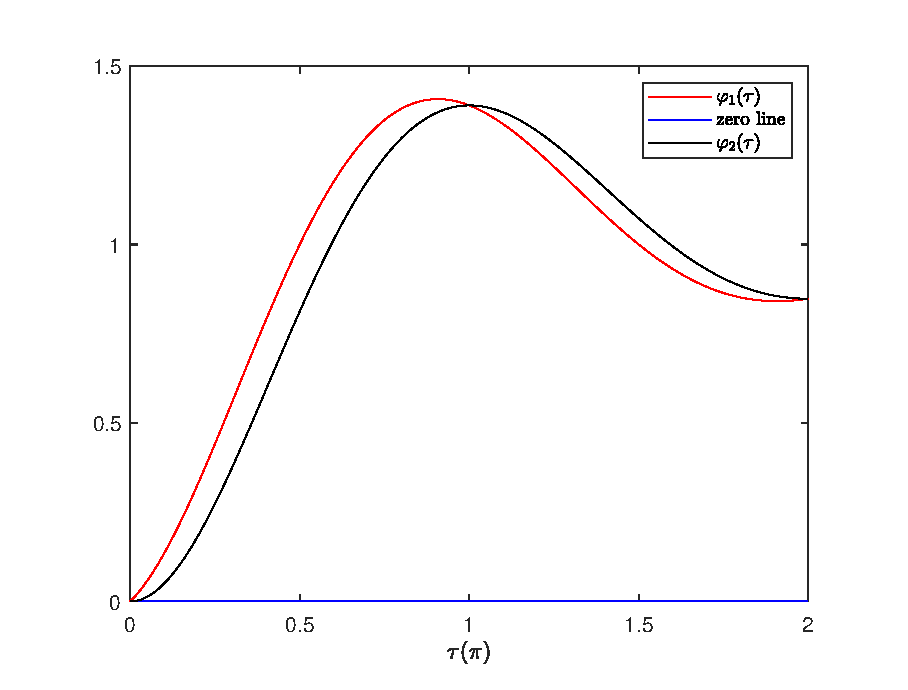
\includegraphics[width= 0.6 \textwidth]{BEB_Explanation/figures/gamma_negative.eps}
				\caption{$\gamma < 0$}
				\label{fig:auxilliary function negative gamma}
			\end{figure}
		%
		
		There is no limit of the evolution time for the point on the boundary to return, actually ($C >0 $)
		$$ 
		\lim_{\tau \rightarrow 0^+} z_0 = - \infty,~\lim_{\tau \rightarrow 0^+} y_0 = +\infty
		$$
		
		$$ 
		\lim_{\tau \rightarrow +\infty} z_0 = + \infty,~\lim_{\tau \rightarrow +\infty} y_0 = -\infty
		$$
		and we can know that 
		\begin{equation}
			\frac{r^+}{r^-}=\frac{1}{C} 
		\left(
			-\lambda + \beta (\gamma^2+1)\frac
			{
				\sin(\tau) {\rm e}^{ \gamma\tau} ({\rm e}^{ \frac{\lambda \tau}{\beta}} - 1)
			}
			{
				\varphi_2^{\gamma}(\tau)
			}
		\right)
		+
		\frac{(C-\lambda)}{C} 
		\frac
		{
			{\rm e}^{(2\gamma + \frac{\lambda}{\beta}) \tau} \varphi_2^{-\gamma}(\tau) 
		}
		{
		\varphi_2^{\gamma}(\tau)
		}
			\label{eq:ratio_r for case alpha notequal lambda}
		\end{equation}
		\begin{align}
			\nonumber
			\frac{z^+}{z^-} &= 
			\frac
			{
				(C-\lambda) N_1 + N_2 + N_3
			}
		%
			{
				(C-\lambda) D_1 + D_2 + D_3
			}
			\label{eq:ratio_Z for case alpha notequal lambda}
		\end{align}
	where 
	$$  
	D_1=
	\left(
	-\cos(\theta )^{2} \gamma \varphi_1^{\gamma}
	+ 
	\gamma  \varphi_3^{\gamma}
	\right),~\varphi_3^{\gamma} = 1-{\rm e}^{\tau  \gamma} (\cos(\tau )+\frac{\sin(\tau )}{\gamma})
	$$
	$$
	D_2 = 
	\beta  (\gamma^{2}+1) 
	\left(
	{\rm e}^{-\frac{\lambda  \tau}{\beta}}-\sin(\theta )^{2}
	\right)
	$$
	$$
	D_3=
	-\beta  \cos(\theta )^{2} 
	\left(
	 1-\varphi_2^{\gamma}(\tau )+\gamma^{2} {\rm e}^{\frac{-\lambda  \tau}{\beta}}
	\right)
	$$
	%
	$$
	N_1 = {\rm e}^{(2\gamma + \frac{\lambda}{\beta}) \tau} D_1(-\gamma)
	$$
	%
	$$
	N_2 = -\beta (\gamma^{2}+1) \cos(\tau)  {\rm e}^{\gamma \tau} \left({\rm e}^{\frac{\lambda \tau}{\beta}}-\sin(\theta)^{2}\right)
	$$
	%
	$$
	N_3 = \beta \cos\! \left(\theta\right)^{2} 
	\left(
	\gamma^{2} {\rm e}^{\frac{\lambda \tau}{\beta}} (1- \varphi_3^{\gamma}(\tau))+1
	\right)
	$$
		Now we should try to know the features of $\frac{r^+}{r^-}$ and $\frac{z^+}{z^-}$:
		
		$$
		\lim_{\tau \rightarrow 0^+} \frac{r^+}{r^-} =1,~ \lim_{\tau \rightarrow +\infty} \frac{r^+}{r^-} = -\frac{\lambda}{C} 
		$$
		
	    $$
		\lim_{\tau \rightarrow 0^+} \frac{z^+}{z^-} =1,
		~ \lim_{\tau \rightarrow \tau_z^-} \frac{z^+}{z^-}  = -\infty ,
		~\lim_{\tau \rightarrow \tau_z^+} \frac{z^+}{z^-}   = +\infty ,
		~\lim_{\tau \rightarrow +\infty} \frac{z^+}{z^-}    = 0
		$$
		$\tau_z$ is the pole of the denominator of $\frac{z^+}{z^-}$, and the bigger $C$ is, the greater $\tau_z$ is, but $\tau_z < 2\pi$.
		
		(2) $\gamma >0$
		
		There is limit of the evolution time ($0<\tau <\pi<\tau_c^2(\gamma)$) for the point on the boundary to return, actually ($C >0 $)
		$$ 
		\lim_{\tau \rightarrow 0^+} z_0 = - \infty,~\lim_{\tau \rightarrow 0^+} y_0 = -\infty
		$$
		
		$$ 
		\lim_{\tau \rightarrow \tau_c^2(\gamma)^-} z_0 = + \infty,~\lim_{\tau \rightarrow \tau_c^2(\gamma)^-} y_0 = +\infty
		$$
		
		Now we should try to know the features of $\frac{r^+}{r^-}$ and $\frac{z^+}{z^-}$:
		
		$$
		\lim_{\tau \rightarrow 0^+} \frac{r^+}{r^-} =1,~ \lim_{\tau \rightarrow \tau_c^2(\gamma)^-} \frac{r^+}{r^-} = +\infty 
		$$
		
		$$
		\lim_{\tau \rightarrow 0^+} \frac{z^+}{z^-} =1,
		~ \lim_{\tau \rightarrow \tau_z(\gamma)^-} \frac{z^+}{z^-}  = +\infty ,
		~\lim_{\tau \rightarrow \tau_z(\gamma)^+} \frac{z^+}{z^-}   = -\infty ,
		~\lim_{\tau \rightarrow +\infty} \frac{z^+}{z^-}    = 0
		$$
		we suppose $De_z(\tau)$ is the denominator of $\frac{z^+}{z^-}$ and 
		$\tau_z$ is the first non-trivial root of the $De_z(\tau)$, and the $\tau_z$ is greater with bigger $C$. By intermediate value theorem, $0< \tau_z < \pi <\tau_c^2$ is true based on  $De_z(0)=0$, $\displaystyle \dot{De_z}(0)= - C(1+\gamma^2 \sin(\theta)^2)<0$ and
		\begin{align}
			\nonumber
			De_z(\pi) &= 
		\beta \gamma^{2} \sin(\theta )^2 \left(1-{\mathrm e}^{\frac{\lambda  \pi}{\beta}}\right)
		+\beta  \left(1-\sin(\theta )^{2} {\rm e}^{\frac{\lambda  \pi}{\beta}}\right) \\
		&+\gamma  (C-\lambda) {\rm e}^{\frac{\lambda  \pi}{\beta}} \sin(\theta )^2 (1+{\rm e}^{\pi  \gamma})
		+\beta  \cos(\theta )^2 {\rm e}^{(\gamma +\frac{\lambda}{\beta}) \pi}
		\end{align}
		is obviously positive for every term is positive.
		
		\begin{figure}[h]
			\centering
			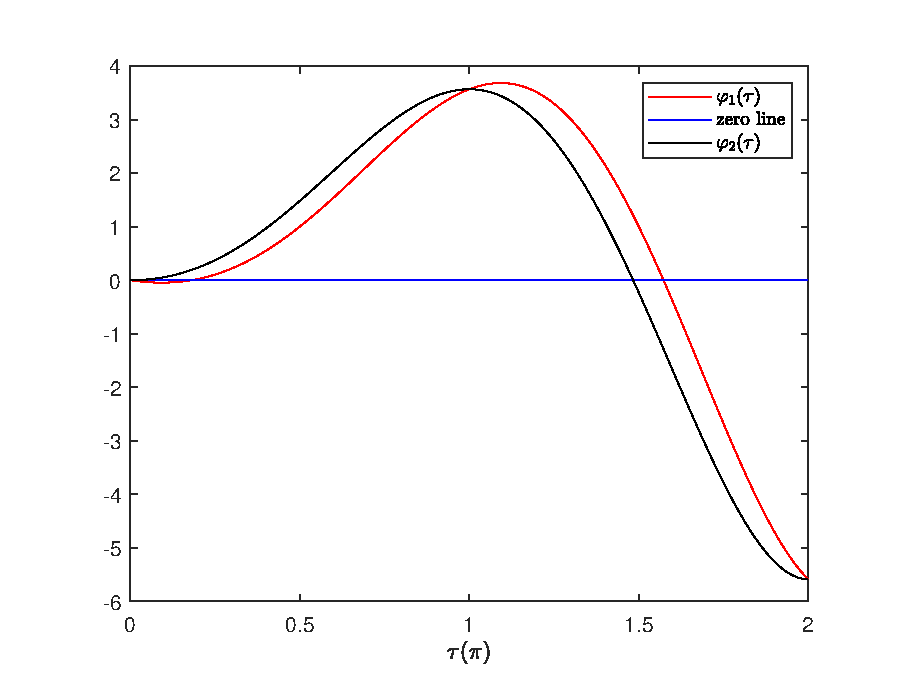
\includegraphics[width= 0.6 \textwidth]{BEB_Explanation/figures/gamma_positive.eps}
			\caption{$\gamma > 0$}
			\label{fig:auxilliary function positive gamma}
		\end{figure}
	\end{enumerate}
	
 	For Example, 
	
	(1) $\alpha = -0.1,~\beta =0.2,~ \gamma = -0.1,~\theta = 0,~R_r=1.5$
	\begin{figure}[h]
		\centering
		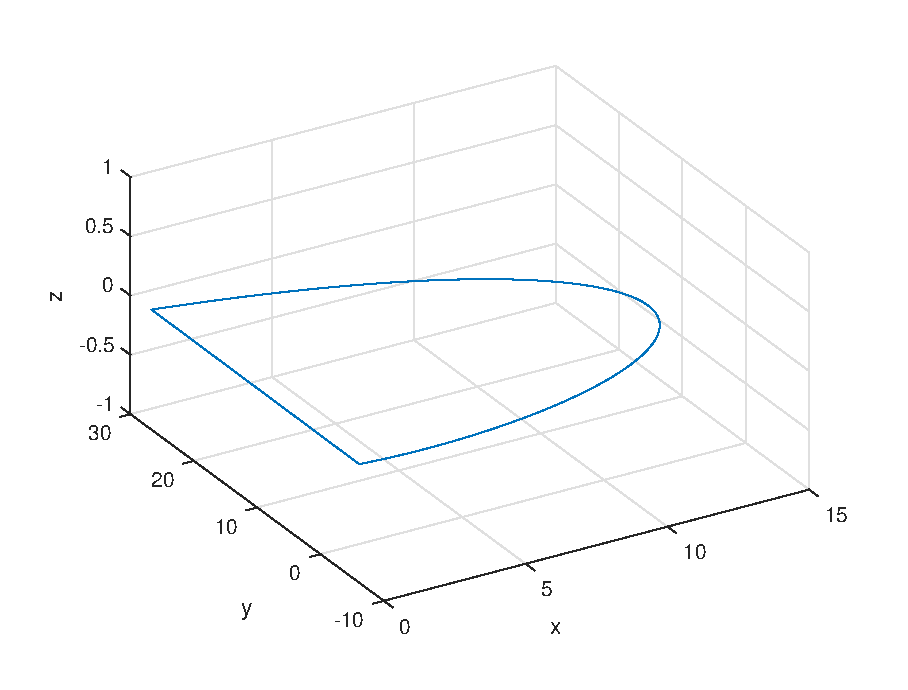
\includegraphics[width= 0.6 \textwidth]{BEB_Explanation/figures/case3_LCO.eps}
		\caption{3D LCO case3}
		\label{fig:3D LCO case3}
	\end{figure}
	
	(2) $\alpha = -0.1,~\beta =0.2,~ \gamma = -0.1,~\theta = \pi/6,~R_r=1.5$
	\begin{figure}[h]
		\centering
		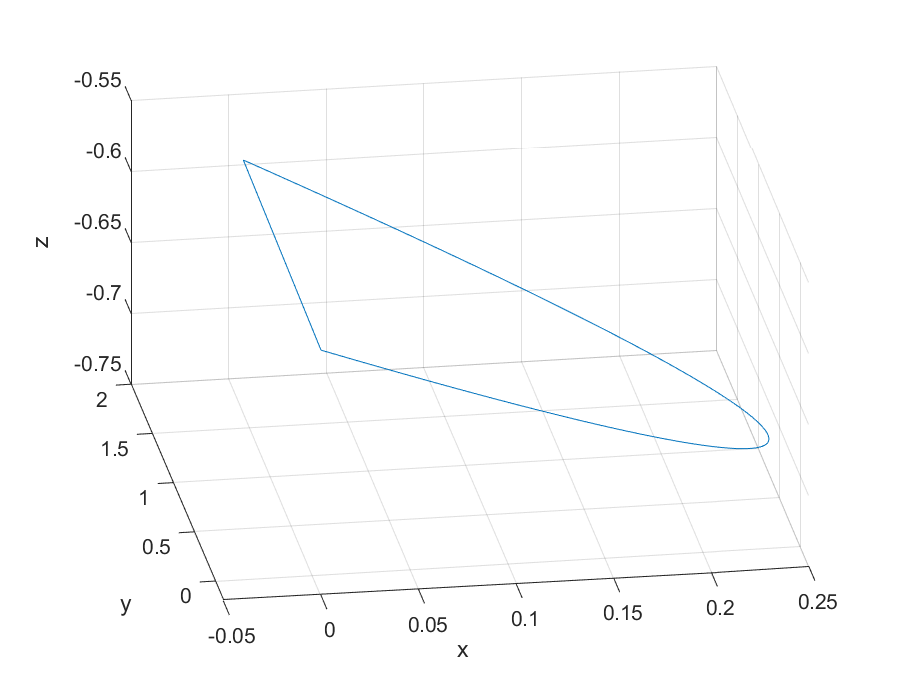
\includegraphics[width= 0.6 \textwidth]{BEB_Explanation/figures/case4_LCO.eps}
		\caption{3D LCO case4}
		\label{fig:3D LCO case4}
	\end{figure}

%
\subsubsection{Boundary equilibrium}

If there is any pseudo equilibrium, it must be on the line $l_3$. The sliding vector field will be 

\begin{equation}
F_s = (\mathbf{I} - \frac{\mathbf{BCA}}{\mathbf{CBA}})\mathbf{A}(x-X_0) = \mathbf{A_s}(x-X_0) 
\end{equation} 

if we set $F_s = 0$, the first equation is just the equation of line $l_3$, and the rank of $\mathbf{A_s}$ is 2, so the firs equation and any one of the left two to solve the pseudo equilibrium point.

$$
X_{pseudo} = 
\begin{bmatrix}
dd
\end{bmatrix}
$$

and the non-trivial eigenvalue of the $\mathbf{A_s}$ is 
\begin{equation}
 \lambda_{s} = \frac
 {
 (1+\varphi_{r}) 
 \left((\gamma+\eta) (1+\sin^{2}(\theta) \gamma^{2})-\gamma \cos^{2}(\theta)
 \right)
 -\varphi_{z} (\gamma^{2}+1) \sin(\theta)	
 }
%
{
(\gamma^{2} \sin^{2}(\theta)+1) (1+\varphi_{r})	
} 
\end{equation}
and we can see that $\lambda_s < 0$ is valid (which means the pseudo equilibrium is stable) if $\varphi_{z}$ satisfies
\begin{equation}
\varphi_{z} > - \frac{ \gamma \cos^{2}(\theta) - 
	(\gamma+\eta) (1+\sin^{2}(\theta) \gamma^{2})
}
{
	(\gamma^{2}+1) \sin(\theta)
}
\end{equation}
%
\begin{figure}[h]
	\centering
	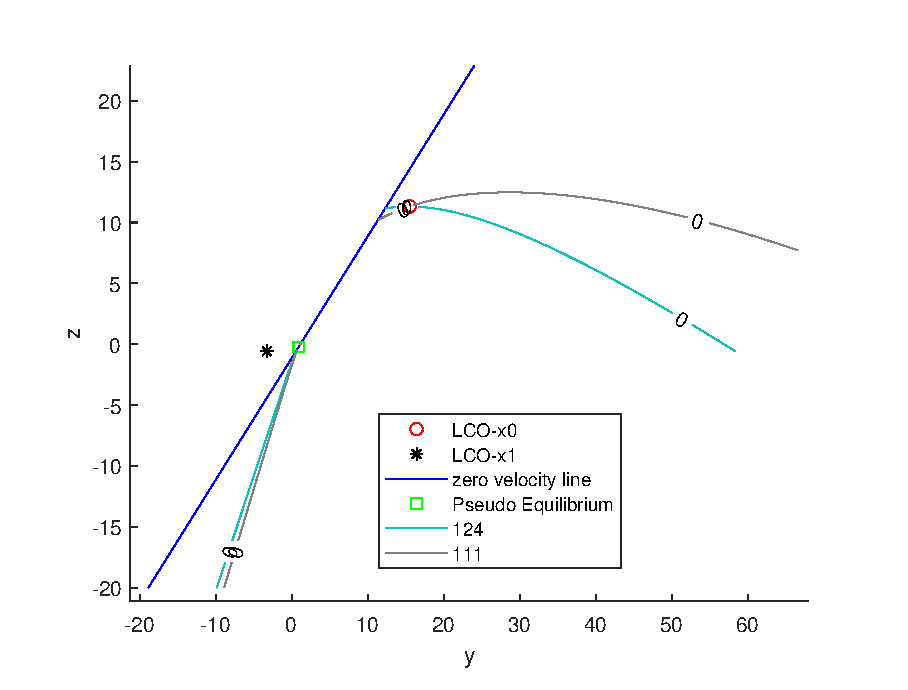
\includegraphics[width= 0.6 \textwidth]{BEB_Explanation/figures/Lyapu_contour.eps}
	\caption{Lyapunov function discrepancy contour}
	\label{fig:Lyapu_contour}
\end{figure}
\subsubsection{Existence of the LCO}
For a general first order ODE like $\dot{y} = \mathbf{A}y$, there is a general solution $y={\rm e}^{\mathbf{A}t} \mathbf{y}_0 $, if $\mathbf V$ and $\mathbf D$ are corresponding eigenvector matrix and eigenvalue matrix of $\mathbf{A}$, we can further get another form 
\begin{align}
	\nonumber
	y & =\mathbf{V} {\rm e}^{\mathbf{D}t} \mathbf{V}^{-1} \mathbf{y}_0\\
	& \mathbf{V} ~diag(\mathbf{V}^{-1} \mathbf{y}_0) \cdot [{\rm e}^{\lambda_1 t},\cdots,{\rm e}^{\lambda_n t}]^{\top}				\\
	&= \mathbf{E} ~\mathbf{S}(t)
\end{align}
where $\mathbf{E} = \mathbf{V} ~diag(\mathbf{V}^{-1} \mathbf{y}_0)$ and $\mathbf{S}(t)=[{\rm e}^{\lambda_1 t},\cdots,{\rm e}^{\lambda_n t}]^{\top}, \mathbf{y} =  \mathbf{x} - \mathbf{x}^0$, and the $\mathbf{x}^0$ is the admissible equilibrium in the region $H(x)<0$.
\begin{figure}[h!]
	\centering
	\includegraphics[width=0.5 \linewidth]{BEB_Explanation/figures/PDM.pdf}
	\caption{Poincar{\' e} map of the LCO}
	\label{fig: poincare map}
\end{figure}
We have known that there is onset of LCO after the boundary equilibrium as iluustrated by Fig.\ref{fig: poincare map}. If we construct a Poincar{\' e} map around $\mathbf{x}_p$  
\[
\Phi\left(\mathbf{x}_p,T^*\right)=\mathbf{x}_p, \quad\left|\mathbf{x}_p \right|>0
\]
With $\beta(T)= E(3,:) S(T), ~ \beta(T^*) = \beta_0$ to implicitly solve the smallest positive value $T^*$. 

Recalling the composed map 
\[
\Phi (\mathbf{x}_0,\tau) =( \varphi \circ R  \circ \varphi) \left(\mathbf{x}_0, \tau(\mathbf{x}_0)\right)  \] ,  where $\mathbf{R} \rightarrow x^{+}=x^- + \mathbf{W} \cdot x^{-}=\mathbf{P} x^-$, $\varphi(x, \tau) $  is flow in linear region.
% And $\varphi (x_{0}, \tau(x_{0})=\mathbf{E}(x_{0}) \cdot \mathbf{S}(\tau(x_{0}))$, $\quad \mathbf{S}(\tau (x_{0}))=\left[{\rm e}^{\lambda_{1} \tau}, \ldots, {\rm e}^{\lambda_{2} \tau}\right]^{\top}$,$\mathbf{E} (x_{0})=V \cdot \operatorname{diag}(\mathbf{V}^{-1} \cdot x_{0}) \quad(E_{n \times n})$. 
From $\mathbf{x}_p$, the time needed  to arrive the impacting surface at $\mathbf{x}_*$ is $t_1$, and then via the reset map, the evolution time from $\mathbf{x}_{**}$ back to $\mathbf{x}_p$ will be $T-t_1$, so the periodic oribit can be constructed by  
\begin{equation} \varphi ( Q(\varphi (\mathbf{x}_p,t_1)),T-t_1)=\mathbf{x}_p
	\label{eq:composed map}
\end{equation}
where the $Q$ is the modified discontinuity map in \cite{Bernardo2007}. 



If we choose the discontinuity boundary as Poincar{\'e} section ($t_1=0$), and we say  the same equation as Eq.\ref{eq:composed map} will be found as 
\begin{equation}
	\mathbf{P}{\rm e}^{\mathbf{A} T^*} (\mathbf{x_{**}}-\mathbf{x}^0) = \mathbf{x_{**}} - \mathbf{x}^0 = \mathbf{y}_{**}
\end{equation}
and obviously the $\mathbf{y_{**}}$ is the eigenvector of matrix $\mathbf{P}{\rm e}^{\mathbf{A} T^*} $ corresponding to the unit eigenvalue, and $\mu \mathbf{y_{**}}$, where $\mu$ is a scalar, is also an eigenvector of the unit eigenvalue, which proves that the ratio between amplitudes of different state variables is the same and linearly dependent to the parameter $\mu$.

In our 3D case, $\mathbf{x}^0 = [-1,0,0]^{\top}$. If we want to find a STABEL LCO, there must a $T^*$ make matrix $\mathbf{P}{\rm e}^{\mathbf{A} T^*} $ have a unit eigenvalue with the  BIGGEST norm, with  eigenvector $\mathbf{y_{**}}=[1,c_1,c_2]^{\top}$ (normalized by first element), obviously the desired starting point of the LCO is $(0,c_1,c_2)$. For all starting points with given evolution $T^*$ to hit the $H(x)=0$ again, they must be on a same line, on the discontinuity surface, $l_t = \{(0,d_1,d_2)|[1,0,0]{\rm e}^{\mathbf{A} T^*} [1,d_1,d_2]^{\top} =[1,0,0]\mathbf{y_{**}} =1  \}$.  We want to find a $T^*$ so that $(0,c_1,c_2)$ is on $l_t$ and simultaneously $\mathbf{y_{**}}=[1,c_2,c_3]^{\top}$ is the eigenvector corresponding to the unit eigenvalue \begin{align}
	\nonumber
	&(\mathbf{P}{\rm e}^{\mathbf{A} T^*} - \mathbf{I})[1,c_2,c_3]^{\top} \\
	\nonumber
	&= \begin{bmatrix}
	f_1(c_1,c_2,T^*)\\
	f_2(c_1,c_2,T^*)\\
	f_3(c_1,c_2,T^*)
	\end{bmatrix}\\
	&=\mathbf{0}
	\label{eq:pseudo Eigenvector equation}
\end{align}
If $f_1=0$ is valid, the  $(0,c_1,c_2)$ is on $l_t(T^*)$;if $f_1 =0$, $f_2 =0$, $f_3 =0$ are all valid then we find our LCO (staring with $(0,c_1,c_2)$), and the it's stable if the biggest norm of eigenvalues is 1, otherwise unstable. 

So we now can construct a numerical scheme to justify the existence of the LCO:

(1) define function $MAX(T) >0$ as the biggest eigenvalue of 
matrix $\mathbf{P}{\rm e}^{\mathbf{A} T^*} $;

(2) use $f_2$ and $f_3$ to solve $c_1(T),~c_2(T)$;

(3) substitute the $c_1(T),~c_2(T)$ got in step 2 into $F_1(T)=f_1(c_1(T),c_2(T),T)$

(4) plot the function $F_1(T)$ and $MAX(T)-1$

Judgments:

$\triangleright$ If there is no $T^*$ let $F_1(T^*)=0$, there will be no LCO;

$\triangleright$ If there is $T^*$ let $F_1(T^*)=0$, there will be a LCO, stable if $MAX(T^*)-1=0$, unstable if $MAX(T^*)-1>0$.

Examples:

(1) $\alpha = -0.1,~\beta =0.2,~ \gamma = -0.1,~\theta = \pi/6,~R_r=0.8,~R_z=0$

\begin{figure}[h!]
	\centering
	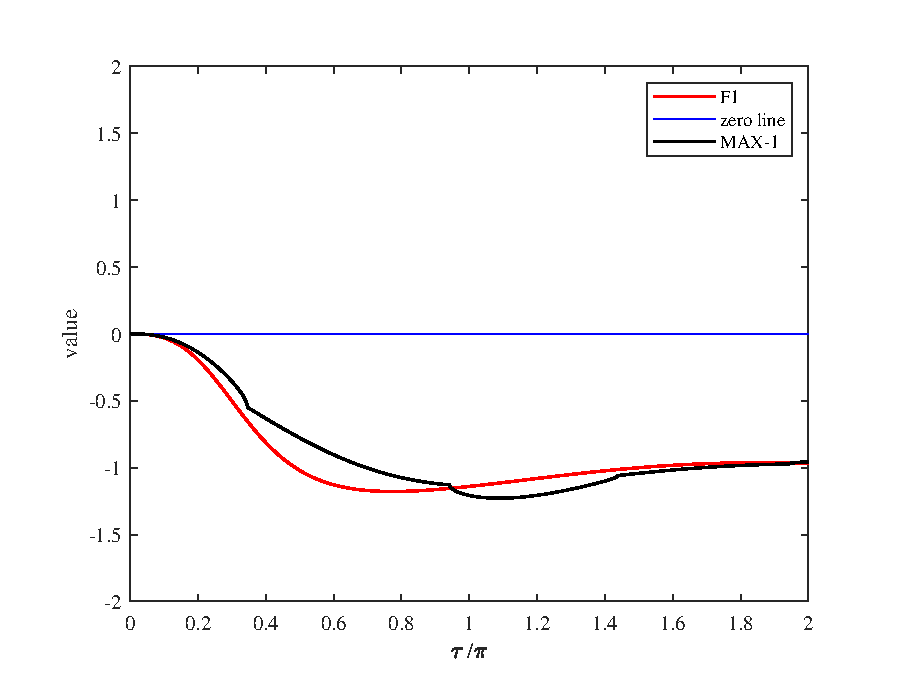
\includegraphics[width=0.5 \linewidth]{BEB_Explanation/figures/class_case1.eps}
	\caption{case 1:No LCO}
	\label{fig: class case1}
\end{figure}

(2) $\alpha = -0.1,~\beta =0.2,~ \gamma = -0.1,~\theta = \pi/6,~R_r=1.5,~R_z=0$

\begin{figure}[h!]
	\centering
	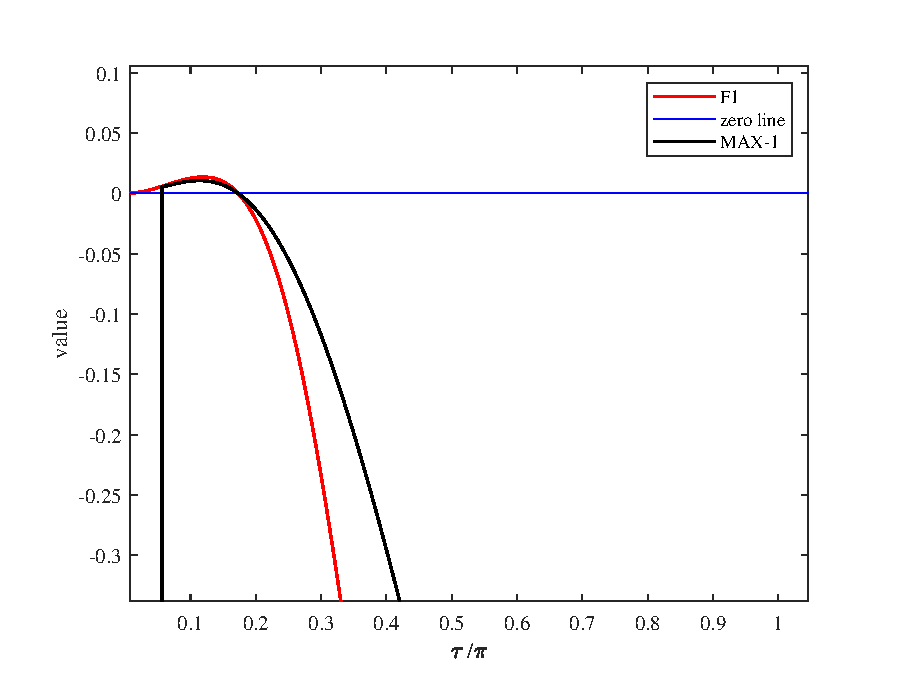
\includegraphics[width=0.5 \linewidth]{BEB_Explanation/figures/class_case2.eps}
	\caption{case 2: LCO}
	\label{fig: class case2}
\end{figure}

(3) $\alpha = -0.1,~\beta =0.2,~ \gamma = -0.1,~\theta = \pi/6,~R_r=0.8,~R_z=4$

\begin{figure}[h!]
	\centering
	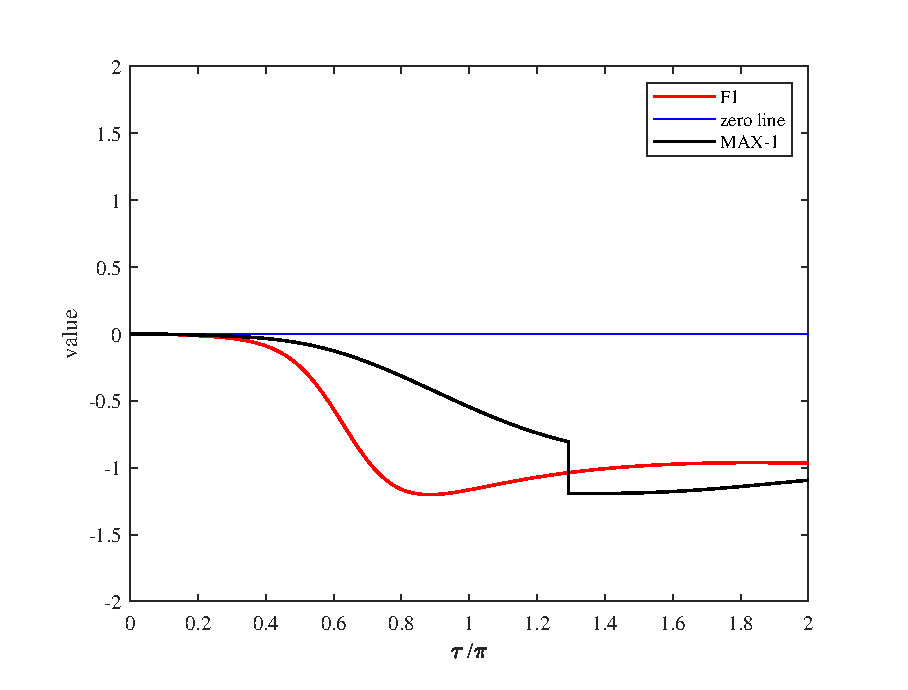
\includegraphics[width=0.5 \linewidth]{BEB_Explanation/figures/class_case3.eps}
	\caption{case 3: No LCO}
	\label{fig: class case3}
\end{figure}

(4) $\alpha = -0.1,~\beta =0.2,~ \gamma = -0.1,~\theta = \pi/6,~R_r=0.8,~R_z=8$

\begin{figure}[h!]
	\centering
	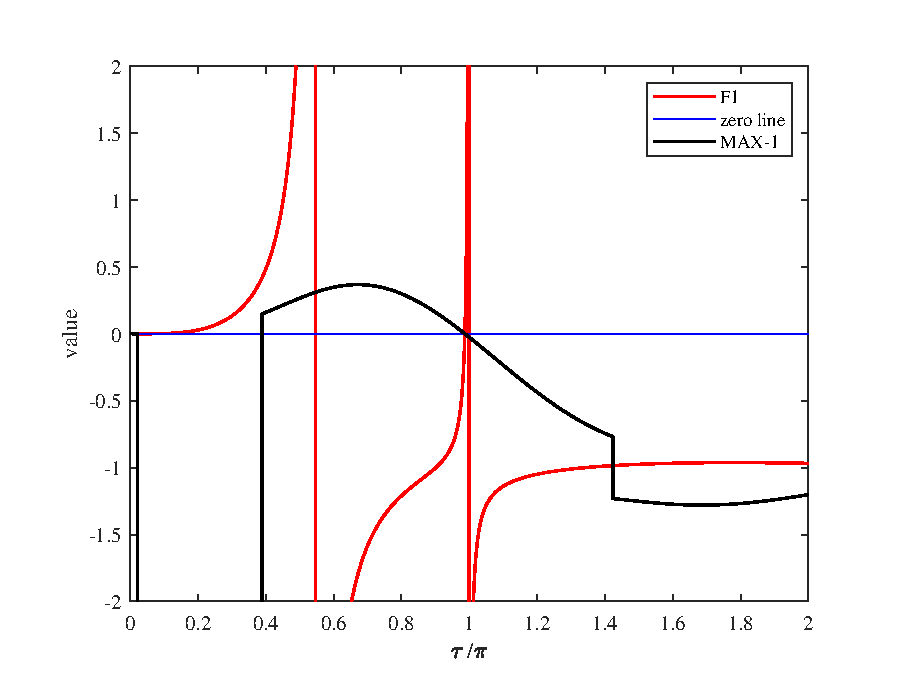
\includegraphics[width=0.5 \linewidth]{BEB_Explanation/figures/class_case4.eps}
	\caption{case 4: LCO}
	\label{fig: class case4}
\end{figure}
\clearpage
Discussion about saltation matrix:
 
To prove the stability of the LCO, we need to find the Jacobi matrix $J^*$ around $\mathbf{x}_p$.
\[ %
J^* = \varphi_x(x_{**},T^*-t_1)~Q_x(x_*)~\varphi_x(x_p,t_1)\]
If we denote matrix function $\mathbf{L}(\mathbf{x}_0)=diag(\mathbf{V}^{-1} \mathbf{x}_0)$, and $\mathbf{L}_{i,i} = \sum_{j=1}^{8}\mathbf{V}_{i,j}^{-1} x_0(j)$ with zeros on non-diagonal positions. Then we observe that  $\frac{\partial \mathbf{L}_{i,i} }{\partial \mathbf{x}_0^{\top}}= \mathbf{V}^{-1}(i,:)$, $\mathbf{E}(i,j) = \mathbf{V}(i,:)\mathbf{L}(:,j)=\mathbf{V}(i,j) \mathbf{L}(j,j)$, which can lead to $$(\mathbf{ES})(i)=\sum_{j=1}^{8} \mathbf{E}(i,j) \mathbf{S}(j)=\sum_{j=1}^{8} \mathbf{V}(i,j) \mathbf{L}(j,j) \mathbf{S}(j)$$ then we can get
\begin{align}
	\frac{\partial (\mathbf{ES})(i)}{\partial (x^*)^{\top}} & = \sum_{j=1}^{8} V(i,j) \frac{\partial L(j,j)}{\partial (x^*)^{\top}}S(j) %+ \sum_{j=1}^{8} V(i,j)L(j,j) \frac{\partial S(j)}{\partial (x^*)^{\top}}
\end{align}
%
furthermore we can write the $\varphi_x$ as
\begin{align}
	\nonumber
	\varphi_x & =  \left( \mathbf{V} diag(\mathbf{S}(T)) 
	\begin{bmatrix}
		\frac{\partial \mathbf{L}_{1,1}}{\partial \mathbf{x}_0^{\top}}\\
		\vdots \\
		\frac{\partial \mathbf{L}_{2,2}}{\partial \mathbf{x}_0^{\top}}
	\end{bmatrix}
	%+
	%\mathbf{E} \frac{\partial \mathbf{S} (T)}{\partial (x^*)^{\top}} 
	\right)
	\\
	& =  \mathbf{V} {\rm e}^{\mathbf{D} T} 
	\mathbf{V}^{-1}
\end{align}

The so-called saltation matrix 
\begin{align}
	\nonumber
	\mathbf{Q}_x (\mathbf{x}_*) &= \mathbf{R}_x(\mathbf{x}_*)+\frac{[F(\mathbf{R}(\mathbf{x}_*))-\mathbf{R}_x(\mathbf{x}_*)F(\mathbf{x}_*)]H_x(\mathbf{x}_*)}{H_x(\mathbf{x}_*)F(\mathbf{x}_*)}\\
	&=\mathbf{P}+ \frac{[F(\mathbf{x}_{**})-\mathbf{P}F(\mathbf{x}_*)]~C}{C~F(\mathbf{x}_*)}
\end{align}
Eventually
\begin{align}
	J^*	 &= \mathbf{V} {\rm e}^{\mathbf{D} (T^*-t_1)} 
	\mathbf{V}^{-1} \mathbf{Q}_x \mathbf{V} {\rm e}^{\mathbf{D} t_1} 
	\mathbf{V}^{-1}\\
	& = \mathbf{V} {\rm e}^{\mathbf{D} (T^*-t_1)} 
	\mathbf{V}^{-1} \left( \mathbf{P}+ \frac{[F(\mathbf{x}_{**})-\mathbf{P}F(\mathbf{x}_*)]~C}{C~F(\mathbf{x}_*)} \right)\mathbf{V} {\rm e}^{\mathbf{D} t_1} 
	\mathbf{V}^{-1}
\end{align}
\end{document}